\head{Февраль}{Листок 6. Метод математической индукции.}

\section{Страдания двоечника Васи.}

В тексте общего характера, как известно читателям книжек про Шерлока Холмса, слово "индукция" означает \textit{"рассуждение от частного к общему"} - в противовес дедукции, \textit{"рассуждению от общего к частному"}. Примеры бытовой индукции часто можно услышать в разговорах: \textit{"У меня было трое знакомых по имени Вася и все они оказались дураками. Ясное дело, все Васи такие"}. Некорректность этого вывода очевидна даже тем, кто никогда не слыхал ни про Жуковского, ни про Тредиаковского. Более корректный вывод про Васю можно найти в анналах средней школы села Липовое.\footnote{Печальная история двоечника Васи была любезно предоставлена нам А.С.Головановым (ГУАСом)}

Жил-был в селе Липовое двоечник Вася. Получал он двойки по всем предметам и в большом количестве. И что бы с ним учителя не делали, от двоек этих никак не мог он избавиться. И так он достал
всех учителей, что решили они навести порядок среди двоек и созвали однажды педсовет, который, как говорят, единогласно принял два решения:
\begin{enumerate}
\item Каждый понедельник ученик Вася Пупкин должен получать двойку.
\item Если учитель видит в журнале, что вчера Вася получил двойку, сегодня ему тоже нужно поставить двойку - так ему, двоечнику!
\end{enumerate}

Интересно, что произойдёт в субботу? Согласно 1. в понедельник Васе двойка обеспечена. Тогда (см. 2.) бедный мальчик получит двойку и во вторник. А раз во вторник, то и в среду. Потом в четверг. Потом в пятницу. Значит, и в субботу!

Представляется интуитивно очевидным, что если бы школу не закрывали в воскресенья и каникулы, череда Васиных двоек продлилась бы бесконечно.

Мы вплотную подошли к осознанию \textit{принципа математической индукции}. В истории про Васю речь идёт о конечном числе шагов. В принципе математической индукции мы оперируем бесконечным
числом шагов. Можно попробовать сформулировать его так:

\fbox{\begin{minipage}{0.95\textwidth}
    Если число 1 обладает некоторым свойством, и вместе с каждым натуральным числом $n$ этим свойством обладает следующее за ним число $n+1$, то этим свойством обладают вообще все натуральные числа.
\end{minipage}} 

\begin{samp}
Если число 1 - хорошее, и из того, что число $n$ - хорошее следует, что число n+1 - хорошее, получаем, что тогда все натуральные числа хорошие. \smiley
\end{samp}

\begin{center}
    \textbf{А теперь просто задача.}
\end{center}

\begin{thm} \label{6.0 thm1}
Из квадрата $16 \cdot 16$ произвольно вырезали одну клетку. Докажите, что полученную фигуру можно разрезать на «уголки» из
трёх клеток.
\end{thm}

{\setlength{\intextsep}{2pt}
\begin{figure}[h]
\begin{minipage}{0.72\linewidth}\setlength{\parindent}{1.5em}
\textbf{\textit{Решение.}} Попытаемся сначала решить более простую аналогичную задачу. 
Во-первых, уменьшим размеры квадрата (например, до $4 \cdot 4$ или $2 \cdot 2$), а, во-вторых, временно зафиксируем вырезанную клетку в углу квадрата. Ну, с квадратом $2 \cdot 2$, вообще всё просто, - какую бы клетку мы не вырезали, оставшиеся три клетки образуют требуемый "уголок" (рис. 1а). А что же делать в квадрате $4 \cdot 4$? Разрежем его на четыре квадратика $2 \cdot 2$. 
\end{minipage}
\hfill
\begin{minipage}{0.25\linewidth}
    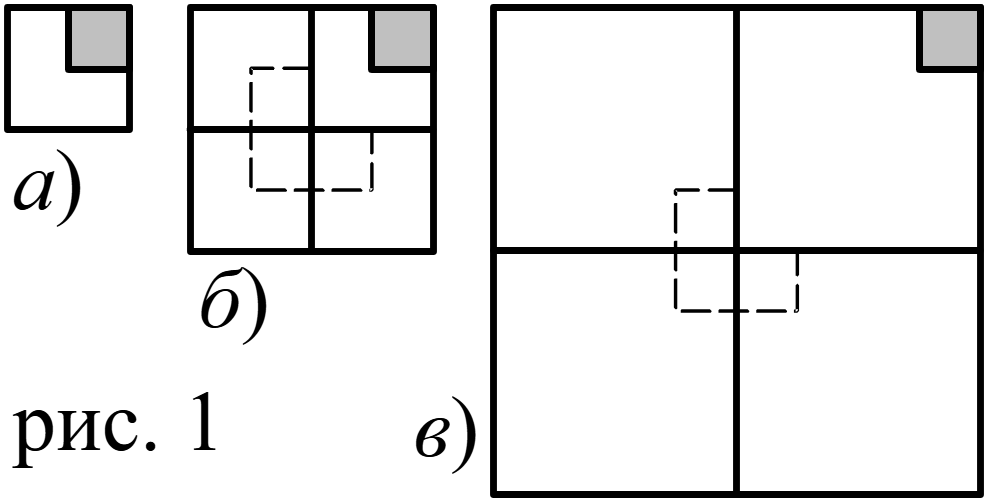
\includegraphics[scale=0.8]{img/kvadrat1.png}
\end{minipage}
\end{figure}}

С тем, у которого имеется вырезанная клетка, всё ясно. Если далее попытаться разрезать оставшийся "большой уголок" на маленькие, то оказывается, что это можно сделать единственным способом (вспомните известную задачу на разрезание уголка из трёх квадратов), причём один из получившихся уголков будет принадлежать всем трем квадратикам $2 \cdot 2$ (рис. 1б), вырезая из каждого именно
угловую клетку. 
Попробуем теперь разрезать на уголки квадрат $8 \cdot 8$ с вырезанным уголком. Делим его на четыре квадрата $4 \cdot 4$: с одним - всё ясно, у остальных вырежем "уголок" из трёх клеток, примыкающих к центру большого квадрата. Каждый из квадратов при этом потеряет по одной клетке, причём опять же
именно по угловой (рис. 1в), а значит, оставшиеся части (как мы уже знаем) можно разрезать на "уголки" из трёх клеток.

{\setlength{\intextsep}{2pt}
\begin{figure}[h]
\begin{minipage}{0.27\linewidth}
    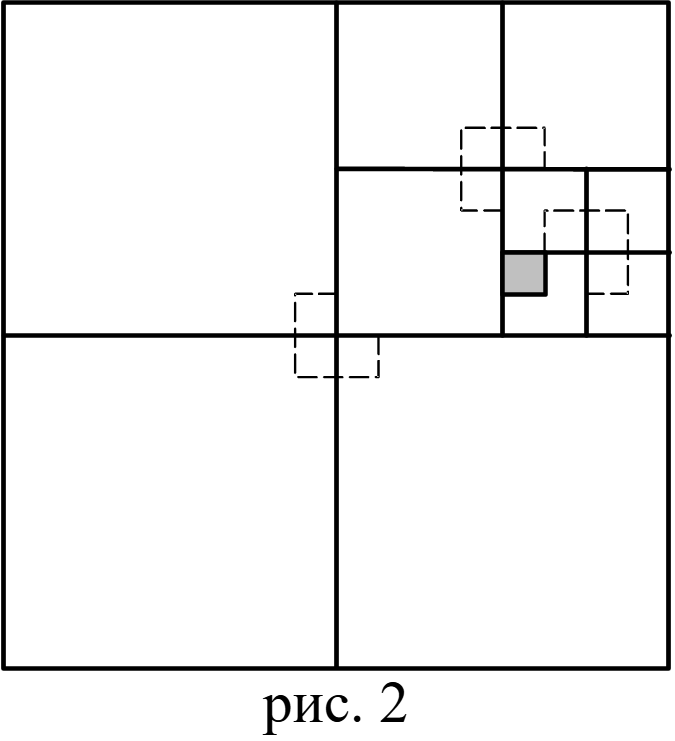
\includegraphics[scale=0.15]{./img/kvadrat2}
\end{minipage}
\hfill
\begin{minipage}{0.72\linewidth}\setlength{\parindent}{1.5em}
    Наверное, все уже поняли, что произойдёт дальше. По аналогичному сценарию мы можем разрезать на требуемые «уголки» и квадрат $16 \cdot 16$, и квадрат $32 \cdot 32$, и т.д. Однако мы забыли, что задача звучала несколько иначе, нежели та, которую мы пока решили, а именно: вырезается из квадрата $16 \cdot 16$ не угловая клетка, а произвольная! Что же делать? 
    \par 
    Довести полученное нами решение до искомого не так уж и трудно. Квадрат $16 \cdot 16$ делим на четыре квадрата $8 \cdot 8$, один из которых (тот, где вырезанная клетка) делим на четыре квадрата $4 \cdot 4$, один из них опять же делим на четыре квадрата $2 \cdot 2$ и начинаем вырезать "уголки". Сначала в том квадратике, где имеется вырезанная клетка, затем "уголки" от трёх
оставшихся квадратиков $2 \cdot 2$, $4 \cdot 4$ и $8 \cdot 8$ (рис. 2). 
\end{minipage}
\end{figure}}

Далее каждый из оставшихся квадратов с вырезанной угловой клеткой мы умеем разрезать на "уголки" из трех клеток. \qed

\textit{\textbf{Обсудим решение.}} Проследим за логикой наших рассуждений. Сначала мы существенно упростили искомую задачу (уменьшили размеры и передвинули, как захотели вырезанную клетку), затем, получив решение самой простой задачи, заметили, что при решении следующей задачи мы можем воспользоваться уже полученным результатом. Далее, как снежный ком - при решении третьей задачи пользуемся результатами второй и так можно продолжать до бесконечности. Ясно, что, идя так по цепочке, мы дойдем до каждого из её утверждений, значит все они верны. Таким образом, мы доказали даже более сильный факт, чем требовалось: любой квадрат $2n \cdot 2n$ без одной клетки можно разрезать на «уголки» из трех клеток.

{\setlength{\intextsep}{2pt}
\begin{figure}[h]
\begin{minipage}{0.45\linewidth}\setlength{\parindent}{1.5em}
Описанный процесс очень напоминает всем знакомую детскую игру - выстраиваешь друг за другом костяшки домино, а затем толкаешь первую. Она повалит вторую, та - третью и так до тех пор, пока не упадут все (рис. 3). Только в наших рассуждениях вместо падающих доминошек - последовательные доказательства утверждений. 
\end{minipage}
\hfill
\begin{minipage}{0.50\linewidth}
    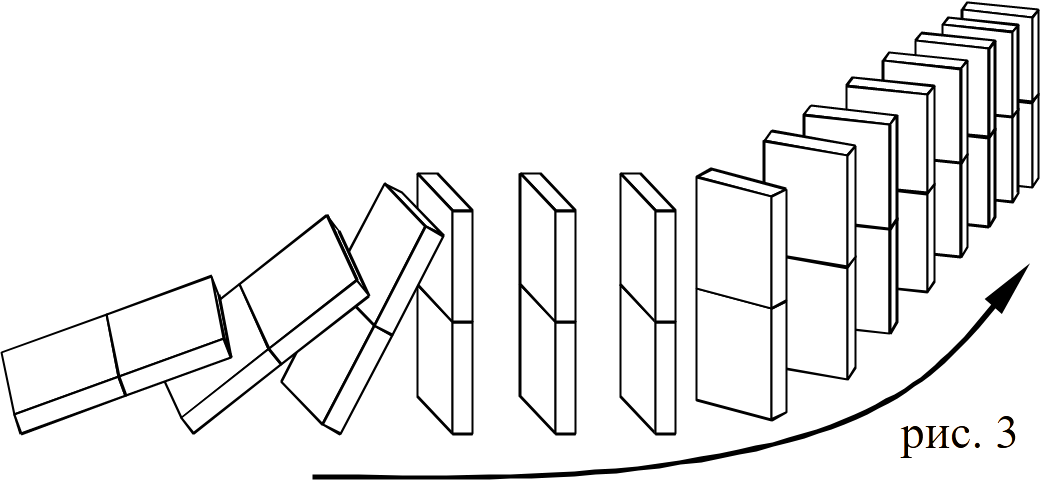
\includegraphics[scale=0.32]{img/domino.png}
\end{minipage}
\end{figure}}
Доказали одно, оно влечёт за собой доказательство следующего, следующее - дальше и т.д.\footnote{Для знатоков: это ещё не индукция в чистом виде. Это пока только рассуждения, подобные индукционным}

\begin{center}
\textbf{Основные определения.}
\end{center}

Прежде чем вводить какие-либо определения заметим, что в предыдущих рассуждениях (задача \ref{6.0 thm1}) все доказываемые утверждения были очень похожи и отличались только степенью двойки в размерах квадрата. Поэтому естественно занумеровать все эти утверждения. 
\par
Первое ($A_1$): квадрат $2^1 \cdot 2^1$ без одной клетки можно разбить на "уголки". 
\par
Второе ($A_2$): квадрат $2^2 \cdot 2^2$ без одной клетки можно разбить на "уголки". 
\par
Третье ($A_3$): квадрат $2^3 \cdot 2^3$ без одной клетки можно разбить на "уголки"...

\begin{ex}
Сформулируйте пятое, семнадцатое и 2012-е утверждения в этой цепочке.
\end{ex}

\begin{ex}
Сформулируйте $n$-е, $(n+1)$-е и $k$-е утверждения в этой цепочке.
\end{ex}

Таким образом, можно представить, что все наши утверждения выстроились в очередь (за доказательством!) друг за другом как "доминошки", а мы приготовились их "толкать". Понятно, надо убедиться, что падая, каждая заденет и увлечёт за собой следующую.

\newpage

\textbf{Основная схема.} Изложенный выше метод рассуждений требует установления истинности двух фактов:

\fbox{\begin{minipage}{0.95\textwidth}
    \textbf{\textit{Факт 1.}} Первое утверждение верно. (мы можем толкнуть первую доминошку)
    \par
    \textbf{\textit{Факт 2.}} Если интересующее нас утверждение верно на каком-то шаге, то верно и следующее за ним утверждение. (толкнув одну, уроним и следующую)
\end{minipage}} 

Первый факт называется \textit{базой (базисом) индукции}, второй - \textit{индукционным переходом} или \textit{шагом индукции}. Индукционный переход включает в себя \textit{посылку (предположение) индукции} (утверждение верно при $n = k$) и \textit{заключение} (утверждение верно при $n = k + 1$). Другими словами, шаг индукции состоит в переходе от посылки к заключению, т.е. в выводе, что заключение верно, если верна посылка. (если упадет $k$-я
доминошка, то упадет и $(k+1)$-я) 

Итак, пусть имеется последовательность утверждений: $A_1$, $A_2$, $...$, $A_n$, $...$ . Для того, чтобы доказать
справедливость \textit{\underline{всех}} утверждений этой последовательности, можно поступить следующим образом:
\begin{enumerate}
\item Доказать истинность утверждения $A_1$;
\item Доказать, что при \textit{\underline{любом}} натуральном $n$ из справедливости утверждения $A_n$ следует справедливость
утверждения $A_n+1$. 
\end{enumerate}

Логический приём, позволяющий заключить, что рассматриваемое утверждение верно для всех натуральных чисел, коль скоро справедливы и базис, и переход называется \textit{методом математической индукции} (ММИ). Утверждения $A_1$, $A_2$, $A_3$, $...$ называют частными формулировками, а утверждение "для всякого $n$ имеет место $A_n$" - универсальной формулировкой. Если мы доказали и базу, и переход, то истинность универсальной формулировки основана на следующем стандартном рассуждении:

\fbox{\begin{minipage}{0.95\textwidth}
    Утверждение $A_1$ истинно, т.к. мы доказали базу индукции. Последовательно применяя индукционный переход при $k$=1, 2, 3, ... , получаем истинность утверждений $A_2$, $A_3$, $A_4$, ... . Этим способом мы можем последовательно дойти до любого значения $n$ и убедиться, что это $A_n$ истинно. Следовательно, для всякого $n$ утверждение $A_n$ справедливо.
\end{minipage}} 

Таким образом, метод математической индукции заключается, по существу, в разрешении не пользоваться стандартным рассуждением в каждой конкретной ситуации, т.е. он позволяет сделать заключение об истинности универсальной формулировки сразу, как только установлена истинность базиса индукции и индукционного перехода.

\section{Доказательство числовых тождеств.}
\epigraph{\textit{"Все равны! Ибо равенство ещё не тождество!"}}{\textit{Афоризм неизвестного автора.}}

\begin{thm}
    Докажите, что при любом натуральном $n$ справедливо равенство 
    \par
    1 + 2 + 3 + ... + $n = \frac{n(n+1)}{2}$
\end{thm}

\begin{prf}
У нас имеется последовательность утверждений:
\par
$A_1 : 1 = \frac{1 \cdot 2}{2}$;
\hfill
$A_2 : 1 + 2 = \frac{2 \cdot 3}{2}$;
\hfill
$A_3 : 1 + 2 + 3  = \frac{3 \cdot 4}{2}$;
\hfill
...
\par
1. \textit{\underline{База индукции:}} очевидно, что утверждение $A_1$ верно.
\par
2. \textit{\underline{Индукционный переход:}} пусть утверждение верно для $n = k$, или, другими словами, пусть верно какое-то
утверждение $A_k$, т.е. верно равенство 1 + 2 + 3 + ... + $k$ = $\frac{k(k+1)}{2}$ (предположение, что $A_k$ верно называется
\textit{индукционным предположением}). Докажем, что тогда утверждение верно и для $n = k +1$, т.е. верно утверждение $A_{k+1}$. Для этого добавим к обеим частям $A_k$ по ($k + 1$):

$1 + 2 + 3 + ... + k + (k + 1) = \frac{k(k+1)}{2} + (k + 1) = \frac{k(k+1)}{2} + \frac{2(k+1)}{2} = \frac{(k+1)(k+2)}{2}$

Но это как раз и есть утверждение $A_{k+1}$. В силу принципа математической индукции верны все утверждения
$A_1$, $A_2$, ... , т.е. наша формула верна при любом натуральном $n$.
\end{prf}

\par

\textbf{\textit{Замечание 1.}} Обращаем ваше внимание, что при выполнении индукционного перехода важно показать, что
все проводимые рассуждения справедливы для любого $k$.

\textbf{\textit{Замечание 2.}} Вместо утверждения $A_1$ в качестве базы индукции мы могли взять, например, утверждение $A_5$. Тогда, выполнив индукционный переход, мы бы доказали, что исходное утверждение верно для всех натуральных $n$, начиная с 5.\footnote{Заметим, что тогда справедливость утверждений 1, 2, 3, 4 мы не доказали и ничего про них не знаем. Такая индукция имеет смысл, если для меньших значений $n$ утверждение не определено. Например, в задачах про многоугольники число сторон не может быть меньше 3, поэтому нет смысла рассматривать утверждения для "двуугольников" или
"одноугольников".}

\begin{thm}
Докажите, что сумма углов выпуклого $n$-угольника равна $180 ^{\circ} \cdot (n-2)$.
\end{thm}

\begin{prf}
Утверждение задачи имеет смысл при всех натуральных $n \geq 3$, поэтому и базой индукции будет соответственно $n = 3$.
\par
\textit{\underline{База}}: утверждение $A_3$ верно по теореме о сумме углов треугольника.
\par
\textit{\underline{Переход}}. выведем заключение о том, что "сумма углов выпуклого ($k$ + 1)-угольника равна $180 ^{\circ} \cdot ((k + 1) - 2) = 180 ^{\circ} \cdot (k -1)$" из предпосылки "сумма углов выпуклого $k$-угольника равна $180 ^{\circ} \cdot (k - 2)$". Для этого в $(k + 1)$-угольнике возьмём две вершины по разные стороны от какой-либо вершины, и соединим их диагональю (это всегда возможно ввиду выпуклости многоугольника)\footnotemark
\end{prf}
\footnotetext{{Существует несколько определений выпуклого многоугольника. В данном случае можно использовать любое из двух: 
    \par
    Первое - "многоугольник называется выпуклым, если для любых двух его точек $A$ и $B$ отрезок $AB$ целиком принадлежит этого многоугольнику". (аналогичным образом можно дать определение любой выпуклой фигуры)
    \par
    Второе - ''многоугольник называется выпуклым, если любая диагональ принадлежит ему целиком''}, которая разобьёт исходный многоугольник на две части: на треугольник и выпуклый $k$-угольник. Сумму углов исходного многоугольника можно получить, сложив сумму углов треугольника ($180 ^{\circ}$) и сумму углов $k$-угольника $(180 ^{\circ} (k-2)$ - индукционное предположение!). Складывая эти суммы, получаем $180 ^{\circ} (k-1)$, что и требовалось доказать.}
    
\section{Задачи на делимость.}

Техника составления и обоснования индукционных переходов при решении задач на делимость похожа на соответствующую технику для тождеств: для доказательства обычно выясняется, КАК изменяется выражение при переходе от $k$ к $k + 1$ и проверяется делимость этого "изменения" на нужное число.

\begin{thm}
Докажите, что $n^3 + (n + 1)^3 + (n+2)^3$ делится на 9 при любом натуральном $n$.
\end{thm}

\begin{prf}
Утверждение задачи имеет смысл при всех натуральных $n \geq 3$, поэтому и базой индукции будет соответственно $n = 3$.
\par
\textit{\underline{База}}: $(n = 1)$: $1^3 + 2^3 + 3^3 = 36$ - делится на 9.
\par
\textit{\underline{Переход}}. пусть при $n = k$ утверждение задачи
истинно (т.е. $k^3 + (k + 1)^3 + (k + 2)^3 \del 9$ при некотором $k$). Докажем тогда, что при $n = k + 1$ утверждение также
справедливо (т.е. $(k + 1)^3 + (k+2)^3 + (k+3)^3 \del 9)$. В самом деле,
\par
\begin{center}
    $(k + 1)^3 + (k + 2)^3 + (k + 3)^3 = \underbrace{(k + 1)^3 + (k + 2)^3 + k^3}_{\mathclap{\del\text{9 по предположению индукции}}} + \underbrace{9k^2 + 27k + 27}_{очевидно \del 9}$
\end{center}
а сумма двух чисел, кратных 9, также кратна 9, что и требовалось доказать.
\par
Тем самым переход доказан и всё утверждение доказано.
\end{prf}

\newpage

\begin{thm}
Докажите, что $47^n + 22$ кратно 23 при любом натуральном $n$.
\end{thm}

\begin{prf}
\par
\textit{\underline{База}} $(n = 1)$: 47 + 22 = 69 - делится на 23. 
\par
\textit{\underline{Переход}}. Пусть при $n = k$ утверждение задачи истинно (т.е. $47^k + 22 \del 23$ при некотором $k$). Докажем тогда, что при $n = k + 1$ утверждение также справедливо (т.е. что $47k + 1
+ 22 \del 23$). В самом деле,
\par
\begin{center}
    $47^{k+1} + 22 = 47^k \cdot 47 + 22 \cdot 47 - 22 \cdot 47 + 22 = 47 \cdot \underbrace{(47^k + 22)}_{\mathclap{\del\text{23 по предположению индукции}}} - \overbrace{(22 \cdot 46)}^{очевидно \del 23}$
\end{center}
а разность двух чисел, кратных 23, также кратна 23, что и требовалось доказать.
\par
Тем самым переход доказан и всё утверждение доказано.
\end{prf}

\vspace*{\fill}

\textbf{\textit{Замечания к листку.}}
\par
Метод математической индукции является серьёзным инструментом для решения задач. Как и любой инструмент перед применением он требует подготовки. В данном конкретном случае подготовка будет заключаться в произнесении "стишка", посвященного ММИ. Помните, что прежде чем начать рассуждение,
вы должны сообщить, по какой переменной вы будете вести индукцию, например, так:
\\
"Будем доказывать методом математической индукции \textit{по n} или \textit{по числу переменных} или \textit{по количеству треугольников} или ..." Далее вы обязаны указать Базу и доказать её. Затем сформулировать индукционное предположение и переход, который собираетесь доказать. Потом доказать переход и завершить доказательство изящной фразой: "Тем самым переход доказан и всё утверждение доказано".

\newpage

\begin{thm}
Докажите, что число 111...11 (243 единицы) делится на 243.
\end{thm}

\begin{prf}\footnote{Заметим, что при решении аналогичных задач возникают типичные ошибки: признака делимости на 27, аналогичного признакам делимости на 3 и на 9 – нет; если число делится на 3 и на 9, то совсем не обязательно, что оно делится на 27.}
Будем доказывать общее утверждение, а именно, что число, записываемое $3^n$ единицами, делится на $3^n$. Индукция по показателю $n$.
\par
\textit{\underline{База}}: 111 делится на 3.  
\par
\textit{\underline{Индукционное предположение}}. Пусть верно для $n = k$, т.е. верно, что число, записываемое $k$ единицами, делится на $3^k$.
\par
\textit{\underline{Переход}}. Докажем для $n = k + 1$. Разделим число, записанное $3^{k+1}$ единицами на число, записанное $3^k$ единицами. Получим число 100..010..01 (две последовательности нулей по $3^k$ - 1 штук). Очевидно, что полученное число делится на 3. Следовательно, исходное число делится на $3^{k+1}$ и тем самым индукционный переход, а, значит, и всё утверждение, доказаны. В частности оно доказано для $n = 5$, поэтому доказано требуемое утверждение, т.к. $243 = 3^5$.
\end{prf}

В предыдущей задаче был осуществлён характерный приём при доказательстве с помощью метода математической индукции, а именно – \textit{обобщение утверждения}. Вместо конкретного утверждения, для конкретного значения длины, количества и т.п. доказывается утверждение \textit{в общем виде}, а требуемое утверждение является частным случаем доказанного. Аналогичный приём был осуществлён в самой первой задаче про разрезание клетчатой доски.

\begin{prf}
В прямоугольнике $3 \cdot 2011$ (2011 столбцов и 3 строки) стоят фишки 3 цветов, по 2011 каждого цвета. Докажите, что можно переставить в каждой строке фишки так, чтобы в каждом столбце были фишки всех трёх цветов.
\end{prf}

{\setlength{\intextsep}{2pt}
\begin{figure}[h]
\begin{minipage}{0.65\linewidth}\setlength{\parindent}{1.5em}
\begin{thm}
На фестивале военно-морской песни собрались 100 хоровых коллективов из разных стран. Каждый хор поёт три песни подряд и тут же уезжает. Жюри, ознакомившись с текстами, выяснило, что каждая песня оскорбительна ровно для одной из стран-участниц. Докажите, что можно составить их расписание выступлений так, чтобы никому не пришлось выслушивать более трех оскорбительных для него песен.
\end{thm}
\end{minipage}
\hfill
\begin{minipage}{0.30\linewidth}
    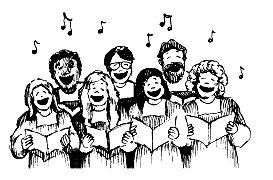
\includegraphics[width=0.95\columnwidth]{img/hor.png}
\end{minipage}
\end{figure}}

\begin{thm}$^{\ast}$
Докажите, что существует 100-значное число, делящееся на 2100, в десятичной записи которого участвуют только цифры 1 и 2.
\end{thm}

\begin{thm}$^{\ast}$
На доске в строчку написаны 100 цифр – нули и единицы (в любой комбинации). Разрешается выполнять два действия: 1) заменять первую цифру (нуль на единицу и единицу на нуль), 2) заменять цифру, стоящую после первой единицы. (Пример: в последовательности 0001101... можно заменить подчёркнутые цифры) Докажите, что с помощью конечного числа таких замен можно получить любую наперёд заданную комбинацию нулей и единиц. 
\end{thm}

\begin{thm}
    Имеется 2011 квадратов. Докажите, что их можно разрезать на части, из которых сложится один квадрат.
\end{thm}

\section{Неравенства.}
\epigraph{\textit{"Равенство двух неравенств возможно только в том случае, когда неравенства идентичны."}}{Афоризм неизвестного автора.}

Приёмы доказательств неравенств более разнообразны, однако, наиболее часто используется следующий факт "сложения неравенств": если $a$ > $b$ и $c$ > $d$, то $a$ + $c$ > $b$ + $d$. Здесь в роли неравенства $a$ > $b$ выступает неравенство для $k$, а $c$ и $d$ – "довески"~к левой и правой частям соответственно при переходе от $k$ к $k + 1$. Кроме того, часто используются промежуточные неравенства. То есть если нужно доказать, что $A$ > $B$, то доказывают, что $A$ > $C$, а затем пользуются тем, что $C$ > $B$.

\begin{thm}
Докажите, что модуль суммы любого числа слагаемых не превосходит суммы модулей этих слагаемых.
\end{thm}

\begin{thm}
Докажите, что при любом натуральном $n$ справедливо неравенство $2n$ > $n$.
\end{thm}

\begin{prf}
\par
\textit{\underline{База}}: $n$ = 1. $2^1 > 1$ - верно.
\par
\textit{\underline{Переход}}. пусть доказано для $n = k$, то есть (\textit{\underline{индукционное предположение}}) пусть верно $2^k > k$. (*) Докажем для $n = k + 1$, то есть докажем, что тогда верно $2^{k+1} > k + 1$.
\par
\textit{1 способ.} Умножим обе части верного по предположению неравенства (*) на 2, получим верное неравенство $2k+1 > 2k$. Но для любого натурального $k$ $2k \geq k + 1$, следовательно, верно, что  $2k + 1 > k + 1$.
\par
\textit{2 способ.} Воспользуемся неравенством, верным для любого натурального $k$: $2k$ > 1. Прибавим к этому неравенству верное по предположению неравенство (*). Получим $2k + 2k > k + 1$. Но выражение в правой части равно $2k + 1$, следовательно, доказано утверждение для $n = k + 1$.
\par
Тем самым переход доказан и всё утверждение доказано. 
\end{prf}

\begin{thm}$^n$ \label{6.0 n1}
Докажите, что при любом натуральном $n$ справедливо неравенство $3n > n + 1$. 
\end{thm}

\begin{thm}
При каких натуральных $n$ выполнено:~а)~$2n > 2n + 1$;~б)~$2n > n^2$~?
\end{thm}

\begin{thm}$^n$ \label{6.0 n2}
Докажите, что при любом натуральном $n$ справедливо неравенство $\frac{(2n)!}{(n!)^2} > \frac{4^n}{n+1}$
\end{thm}

\begin{thm}$^\ast$
Докажите, что при любом натуральном $n$, начиная с 2, справедливо неравенство: 	
\par \begin{center}
    $2^n > 1 + n \sqrt{2^{n-1}}$
\end{center} \end{thm}

\begin{thm}
Докажите, что при любом натуральном $n$, начиная с 2, справедливо неравенство: 
\par \begin{center}
    $\frac{1}{n + 1} + \frac{1}{n+2} + ... + \frac{1}{2n} > \frac{13}{14}$.
\end{center} \end{thm}

\begin{thm}
Докажите \textit{неравенство Бернулли}: $(1 + х)^n \geq 1 + nx$ при $х \geq –1, n \in \mathbb{N}$.
\end{thm}

\begin{thm}
Докажите, что при любом натуральном $n$ справедливо неравенство $1 + \frac{1}{2} + \frac{1}{4} + ... + \frac{1}{2^n} < 2$.
\end{thm}

\begin{prf} Докажем неравенство индукцией по $n$.
\par
\textit{\underline{База}}: $(n = 1)$. $1 + \frac{1}{2} < 2$ верно.
\par
\textit{\underline{Индукционное предположение}}. Пусть верно для $n = k$, то есть верно, что $1 + \frac{1}{2} + \frac{1}{4} + ... + \frac{1}{2^k} < 2$. ($\circ\circ$)
\par
\textit{\underline{Переход}}. Докажем для $n = k + 1$, то есть докажем, что тогда верно $1 + \frac{1}{2} + \frac{1}{4} + ... + \frac{1}{2^k} + \frac{1}{2^{k+1}} < 2$. ($\circ\circ\circ$) Разделим обе части неравенства ($\circ\circ$) на 2. Получим: $\frac{1}{2} + \frac{1}{4} + ... + \frac{1}{2^k} + \frac{1}{2^{k+1}} < 1$. Прибавляя к обеим частям этого неравенства по 1, получаем неравенство ($\circ\circ\circ$). Тем самым переход доказан и требуемое неравенство доказано. 
\end{prf}

\newpage

\section{Парадокс изобретателя.}

{\setlength{\intextsep}{2pt}
\begin{figure}[h]
\begin{minipage}{0.74\linewidth}\setlength{\parindent}{1.5em}
Попробуем доказать при помощи метода математической индукции два неравенства:
\par
\begin{equation*}
  1)~\frac{1}{2} \cdot \frac{3}{4} \cdot ... \cdot \frac{2n - 1}{2n} < \frac{1}{\sqrt{n}} ~~~и~~~
  2)~\frac{1}{2} \cdot \frac{3}{4} \cdot ... \cdot \frac{2n - 1}{2n} < \frac{1}{\sqrt{n + 1}}
\end{equation*}

\par
Базис индукции проверяется без труда
\begin{equation*}
  1)~ \frac{1}{2} < \frac{1}{1} = \frac{1}{\sqrt{1}} ~~~и~~~   
  2)~ \frac{1}{2} < \frac{1}{\sqrt{2}} = \frac{1}{\sqrt{1 + 1}}
\end{equation*}
\par
По предположению индукции, мы имеем
\begin{equation*}
  1)~\frac{1}{2} \cdot \frac{3}{4} \cdot ... \cdot \frac{2k + 1}{\sqrt{2k + 2}} = \frac{1 \cdot 3 \cdot ... \cdot (2k - 1)}{2 \cdot 4 \cdot ... \cdot 2k} \cdot \frac{2k + 1}{2k + 2} < \frac{1}{\sqrt{k}} \cdot \frac{2k + 1}{2k + 2}
\end{equation*}
$$и$$
\begin{equation*}
  2)~\frac{1}{2} \cdot \frac{3}{4} \cdot ... \frac{2k + 1}{\sqrt{2k + 2}} = \frac{1 \cdot 3 \cdot ... \cdot (2k - 1)}{2 \cdot 4 \cdot ... \cdot 2k} \cdot \frac{2k + 1}{2k + 2} < \frac{1}{\sqrt{k + 1}} \cdot \frac{2k + 1}{2k + 2}
\end{equation*}

\end{minipage}
\hfill
\begin{minipage}{0.25\linewidth}
    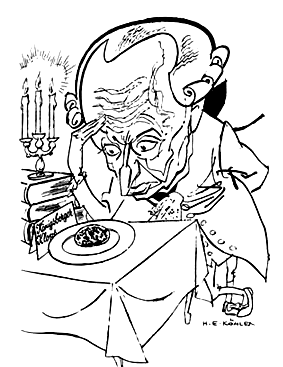
\includegraphics[width=0.95\columnwidth]{img/euler_k.png}
\end{minipage}
\end{figure}}

\par
нам остаётся доказать, что
\begin{equation*}
1)~\frac{1}{\sqrt{k}} \cdot \frac{2k + 1}{2k + 2} \leq \frac{1}{\sqrt{k + 1}}
   ~~~и~~~    
  2)~\frac{1}{\sqrt{k + 1}} \cdot \frac{2k + 1}{2k + 2} \leq \frac{1}{\sqrt{k + 2}}
\end{equation*}

\par
Возводя обе части неравенства в квадрат, избавляясь от знаменателей и раскрывая скобки, 
\par
приходим к эквивалентным неравенствам
\begin{equation*}
1)~4k^3 + 8k^2 + 5k + 1 \leq 4k^3 + 8k^2 + 4k
 ~~~и~~~
  2)~4k^3 + 12k^2 + 9k + 2 \leq 4k^3 + 12k^2 + 12k + 4
\end{equation*}

Вспоминая, что число $k$ натуральное, легко убедиться, что левое неравенство неверно, а правое верно. Но как же так оказалось? Ведь правое неравенство сильнее (!), и из него автоматически следует левое. Дело в том, что хотя во втором случае нам и пришлось доказывать более сильное заключение, но одновременно с этим мы могли пользоваться и более сильным предположением индукции. При этом, ни в коем случае нельзя считать первое неравенство неверным. Наша неудача в нём говорит лишь о том, что не годится конкретный метод доказательства – математическая индукция. 
\par
Подобная ситуация получила название \textit{парадокс изобретателя}.\footnote{На рисунке приведена карикатура на Иммануила Канта (1724 – 1804). Современные кенигсбержцы достаточно хорошо знают великого земляка Иммануила Канта. Он известен как философ и как профессор Кенигсбергского университета, написавший большое количество философских работ, в том числе изданную на русском языке «Критику чистого разума».
Но Кант известен не только как философ и преподаватель, но и как простой человек, имеющий свои слабости. Известен он также и как педант, как человек, не покидавший Кенигсберг всю свою жизнь и дальше его окрестностей не выезжавший. Но мало кто знает, что он еще прославился и как изобретатель, достигнув высот, которые если не уравнивают его с Леонардо да Винчи, то, по крайней мере, ставят его в один ряд со многими изобретателями мирового значения. Кто бы мог предположить, что такой обыденный канцелярский прибор, как дырокол впервые был придуман и использован Кантом. Единственное отличие от современного дырокола, имеющего отверстие 5 мм, является то, что Кант использовал аналогичный прибор с отверстием 11,6 мм. По этому диаметру отверстия всегда можно определить дырокол, изобретенный Кантом. До середины 19 века не было документов, которые имели бы такие аккуратные отверстия, кроме документов Иммануила Канта. Первые листы, подшитые к делу с отверстием 11,6 мм, обнаружили советские исследователи в 1956 году. Они датировались декабрем 1799 г., и эта дата была объявлена датой первого употребления дырокола, изобретенного Кантом. Но через пять лет уже в Германии были обнаружены бумаги Канта с отверстием диаметром 11,6 мм за октябрь 1787 г. И дата первого употребления дырокола в канцелярском мире сдвинулась на 12 лет...
\par
При опросе работников канцелярий оказалось, что 75\% из них знают Иммануила Канта только как изобретателя дырокола; 5\% – что он еще является философом, и 2\% – что он еще преподавал в Кенигсбергском университете. Остальные 18\% вообще ничего не слышали о Канте. \smiley}

\par
Парадокс изобретателя предложил нам ещё одну идею доказательства неравенств, а именно – усиление утверждения. Примером такого метода может служить задача: "Докажите неравенство $\frac{1}{2} \cdot \frac{3}{4} \cdot ... \cdot \frac{2n - 1}{2n} < \frac{1}{\sqrt{n}}$." Вместо доказательства требуемого неравенства мы доказываем по индукции более сильное неравенство $\frac{1}{2} \cdot \frac{3}{4} \cdot ... \cdot \frac{2n - 1}{2n} < \frac{1}{\sqrt{n + 1}}$.", а затем пользуемся тем, что $\frac{1}{\sqrt{n+1}} < \frac{1}{\sqrt{n}}$. Разберём еще один пример.